\section{Tilt-Angle Branch Structure and MFG-Directed Continuations}
\label{app:tilt_sign_branch_mfg_alignment}

The folded representation in Fig.~\ref{fig:bloch_disk_portrait}(b) compresses the transverse sign and
therefore hides part of the qubit geometry.  The result is a visually suggestive ``reflection'' that is easy to
misread as a dynamical reversal.  The physically cleaner interpretation is a two-part statement:
\begin{enumerate}
    \item the reduced-state tilt angle is a chart variable extracted through an inverse tangent and is therefore
    branch-valued;
    \item the sign of the tilt-angle argument itself depends on a competition between thermal and coupling-driven
    scales.
\end{enumerate}
Once these are separated, the branch family that aligns with the Cresser--Anders ultrastrong mean-force Gibbs
(MFG) endpoint is the continuation that lands on the coupling-direction sector, not the branch that returns to the
bare ground-state ray.

\paragraph{Exact geometry and what is actually singular.}
In the rewritten qubit parameterization (Sec.~\ref{subsec:qubit_exact_geometry}) the reduced-state magnetisation
in the $(\hat{\mathbf e}_{\perp}^{(s)},\hat{\mathbf n}_s)$ plane is
\begin{align}
    m_z &= \tanh\Theta,
    \\
    m_\perp &= \tan\eta\left(m_z\cosh a+\sinh a\right),
    \qquad a\equiv \beta\omega_q/2,
    \label{eq:tilt_sign_branch_mz_mperp}
\end{align}
with
\begin{equation}
    \tan\eta=-\cot\theta\,\frac{\Sigma_\perp}{\Sigma_z}.
    \label{eq:tilt_sign_branch_taneta}
\end{equation}
The principal tilt-angle chart is defined by
\begin{equation}
    \tan\varphi
    =-\frac{m_\perp}{m_z}
    =-\tan\eta\left(\cosh a+\sinh a\,\coth\Theta\right).
    \label{eq:tilt_sign_branch_tanphi}
\end{equation}
The Cartesian Bloch vector $(m_\perp,m_z)$ is the physical object.  The singularity is in the \emph{chart}
variable $\varphi$ (through the inverse tangent), not in the state itself.

\paragraph{A rational form for the tilt-angle argument.}
Define
\begin{equation}
    \tan\varphi = X(\beta,g,\theta),
    \qquad
    X \equiv \cot\theta\,\frac{\Sigma_\perp}{\Sigma_z}
    \left(\cosh a+\sinh a\,\coth\Theta\right).
    \label{eq:tilt_sign_branch_X}
\end{equation}
With $s\equiv \sin\theta$ and
\begin{equation}
    u\equiv \gamma s^2\Sigma_z,
    \qquad
    t_a\equiv \tanh a,
    \qquad
    \Theta=\operatorname{arctanh}(u)-a,
    \label{eq:tilt_sign_branch_u_ta_def}
\end{equation}
one has
\begin{equation}
    \tanh\Theta=\frac{u-t_a}{1-u t_a}
    \quad\Longrightarrow\quad
    \coth\Theta=\frac{1-u t_a}{u-t_a},
    \label{eq:tilt_sign_branch_coth_exact}
\end{equation}
and therefore
\begin{equation}
    \cosh a+\sinh a\,\coth\Theta
    =
    \frac{u\,\mathrm{sech}\,a}{u-t_a}.
    \label{eq:tilt_sign_branch_hyperbolic_factor_rational}
\end{equation}
Substituting this into Eq.~\eqref{eq:tilt_sign_branch_X} yields the exact rationalized form
\begin{equation}
    X
    =
    \cot\theta\,\frac{\Sigma_\perp}{\Sigma_z}\,
    \frac{u\,\mathrm{sech}\,a}{u-t_a}
    =
    \cot\theta\,\gamma s^2\Sigma_\perp\,
    \frac{\mathrm{sech}\,a}{u-t_a}.
    \label{eq:tilt_sign_branch_X_rational}
\end{equation}

This is the key simplification.  The numerator carries the transverse sign through $\Sigma_\perp$, while the
denominator carries the thermal--coupling competition through
\begin{equation}
    u(\beta,g)-\tanh a(\beta).
    \label{eq:tilt_sign_branch_scale_competition}
\end{equation}
Thus the sign of the tilt-angle argument is controlled by the \emph{relative scaling} of $\beta$ and $g$:
\begin{equation}
    \mathrm{sgn}\,X
    =
    \mathrm{sgn}(\cot\theta)\,
    \mathrm{sgn}(\Sigma_\perp)\,
    \mathrm{sgn}\!\bigl(u-\tanh a\bigr).
    \label{eq:tilt_sign_branch_signX}
\end{equation}
The chart enhancement occurs when $u\approx \tanh a$ (equivalently $m_z\approx 0$), but sign changes can also be
triggered by $\Sigma_\perp$ changing sign.  These are distinct mechanisms.

\paragraph{Continuous angle branches and the geometric hub.}
The continuous vector-angle branch is
\begin{equation}
    \varphi_{\rm cont}=\arctan X+n\pi,
    \qquad n\in\mathbb Z,
    \label{eq:tilt_sign_branch_phi_cont}
\end{equation}
while the axis-angle chart identifies $\varphi$ and $\varphi+\pi$.  For the unfolded Bloch-circle plots it is
useful to define the axis angle
\begin{equation}
    \varphi_{\rm ax}\equiv \varphi \pmod{\pi}.
\end{equation}
In the plotting convention used here (angle measured from the bare ground-state ray $-\hat{\mathbf n}_s$ toward
the positive transverse direction), the coupling-axis ray is $\pi-\theta$.  The visible branch-selection geometry
is therefore organized by the \emph{hub condition}
\begin{equation}
    \varphi_{\rm ax}=\pi-\theta \quad (\mathrm{mod}\ \pi),
    \label{eq:tilt_sign_branch_hub_condition}
\end{equation}
which need not coincide with the principal-chart singularity $u=\tanh a$.

Near the hub, the local branch family is naturally two-valued on the axis chart,
\begin{equation}
    \varphi_{\rm ax}^{(+)}\sim \pi-\theta,
    \qquad
    \varphi_{\rm ax}^{(-)}\sim \theta,
    \label{eq:tilt_sign_branch_two_images}
\end{equation}
and four-valued on a lifted vector chart through parity shifts,
\begin{equation}
    \varphi_{\rm cont}^{(\pm)}+\pi.
    \label{eq:tilt_sign_branch_four_images}
\end{equation}
This is the source of the ``two or four branches'' language: a single geometric hub together with sign
multiplicity and inverse-tangent sheet choice.

\paragraph{Which branch is physically relevant for MFG alignment?}
The ultrastrong MFG state quoted by Cresser and Anders for a qubit coupled along $\hat{\mathbf r}$ is
\begin{equation}
    \rho_S^{(\lambda\to\infty)}
    =
    \frac12\Bigl[\mathbf 1-\sigma_{\hat{\mathbf r}}
    \tanh\!\bigl(\tfrac12\beta\omega_q\cos\theta\bigr)\Bigr].
    \label{eq:tilt_sign_branch_cresser_anders_mfg}
\end{equation}
In our notation $\hat{\mathbf r}\equiv \hat{\mathbf f}$.  The MFG-compatible branch is therefore the
continuation whose endpoint lies on the \emph{coupling-direction sector} (the $\theta$ ray in the plotting
convention), not the continuation that returns to the bare ground-state ray.

This can be made explicit by comparing the exact equilibrium ultrastrong endpoint to the MFG target.  From
Appendix~\ref{app:branch_alignment_codex},
\begin{equation}
    \Theta(\chi)=\operatorname{arctanh}\!\bigl(\cos\eta\,\tanh\chi\bigr)-a,
    \qquad a=\beta\omega_q/2,
    \label{eq:tilt_sign_branch_Theta_of_chi_eta}
\end{equation}
so at fixed $(\beta,\theta)$,
\begin{equation}
    \Theta_\infty=\lim_{g\to\infty}\Theta=\operatorname{arctanh}(\cos\eta)-a,
    \label{eq:tilt_sign_branch_Theta_infty}
\end{equation}
because $\chi=g^2\chi_0\to\infty$ implies $\tanh\chi\to 1$.  Substituting into
Eq.~\eqref{eq:tilt_sign_branch_mz_mperp} gives the exact equilibrium ultrastrong endpoint
\begin{equation}
    \mathbf m_{\infty}^{\rm(ex)}
    =
    \frac{
        \sin\eta\,\hat{\mathbf e}_{\perp}^{(s)}
        +
        \bigl(\cos\eta\cosh a-\sinh a\bigr)\hat{\mathbf n}_s
    }{
        \cosh a-\cos\eta\,\sinh a
    },
    \label{eq:tilt_sign_branch_exact_ultrastrong_vector}
\end{equation}
with exact purity
\begin{equation}
    r_{\infty}^{\rm(ex)}=\lim_{g\to\infty}\tanh\chi=1.
    \label{eq:tilt_sign_branch_exact_ultrastrong_pure}
\end{equation}

By contrast, the MFG endpoint in our notation is
\begin{equation}
    \rho_{S,\infty}^{\rm(MFG)}
    =
    \frac12\bigl[\mathbf 1-\sigma_{\hat{\mathbf f}}\,r_{\rm MFG}\bigr],
    \qquad
    r_{\rm MFG}\equiv \tanh(a\cos\theta),
    \label{eq:tilt_sign_branch_mfg_reparam}
\end{equation}
so MFG consistency requires both
\begin{align}
    \varphi_{\rm ax}^{\rm(br)}(g\to\infty) &= \theta \quad (\mathrm{mod}\ \pi),
    \label{eq:tilt_sign_branch_mfg_angle_condition}
    \\
    r_{\rm br}(g\to\infty) &= \tanh(a\cos\theta).
    \label{eq:tilt_sign_branch_mfg_radius_condition}
\end{align}
Equation~\eqref{eq:tilt_sign_branch_exact_ultrastrong_pure} then shows the obstruction directly: a pure chart
relabeling can match the \emph{direction}, but not the finite-temperature MFG \emph{radius}.

\paragraph{Correlated-limit viewpoint and branch selection.}
The physically persuasive way to state the MFG comparison is to keep the effective thermal variable
\begin{equation}
    a_{\rm eff}\equiv \frac{\beta\omega_q}{2}\cos\theta
    \label{eq:tilt_sign_branch_aeff}
\end{equation}
visible in the asymptotic endpoint.  Then the MFG radius is simply
\begin{equation}
    r_{\rm MFG}=\tanh a_{\rm eff},
    \label{eq:tilt_sign_branch_rMFG_beta}
\end{equation}
with density-matrix purity
\begin{equation}
    \mathcal P_{\rm MFG}=\frac12\bigl(1+r_{\rm MFG}^2\bigr).
    \label{eq:tilt_sign_branch_PMFG_beta}
\end{equation}
In this correlated-limit language the endpoint radius is fixed by $a_{\rm eff}$, and the remaining freedom is
angular.  The two post-hub continuations therefore correspond to distinct endpoint directions:
\begin{align}
    \mathbf m_{\rm br}^{\rm(ground)} &\to -\,\tanh(a_{\rm eff})\,\hat{\mathbf n}_s,
    \label{eq:tilt_sign_branch_ground_endpoint_aeff}
    \\
    \mathbf m_{\rm br}^{\rm(MFG)} &\to -\,\tanh(a_{\rm eff})\,\hat{\mathbf f}.
    \label{eq:tilt_sign_branch_f_endpoint_aeff}
\end{align}
The second is the Cresser--Anders-compatible branch.  In other words: once the endpoint is required to retain a
finite thermal imprint through $a_{\rm eff}$, the continuation that runs back to the bare ground state is no
longer the physically relevant branch for MFG matching.

A simple branch-family ansatz implementing this idea is
\begin{equation}
    \mathbf m_{\rm br}(\beta)
    =
    r_{\rm MFG}(\beta)\,
    \bigl[\sin\alpha_{\rm br}(\beta)\,\hat{\mathbf e}_{\perp}^{(s)}
          -\cos\alpha_{\rm br}(\beta)\,\hat{\mathbf n}_{s}\bigr],
    \label{eq:tilt_sign_branch_mfg_guided_ansatz}
\end{equation}
where $\alpha_{\rm br}(\beta)$ is selected from the local branch family so that the trajectory passes through the
hub and asymptotes to the $\theta$ sector.  This is a branch-switched continuation rule, not an exact
equilibrium trajectory.

\paragraph{Purity diagnostics: exact law versus branch-switched families.}
For the exact equilibrium qubit state,
\begin{equation}
    r_{\rm exact}(\beta,g)=\sqrt{m_z^2+m_\perp^2}=\tanh\chi(\beta,g).
    \label{eq:tilt_sign_branch_exact_purity}
\end{equation}
If one only relabels the angle chart, the purity is unchanged.  If one instead reconstructs a new branch-switched
state trajectory, the purity becomes an independent diagnostic:
\begin{equation}
    r_{\rm br}(\beta)\equiv
    \sqrt{\bigl[m_z^{\rm(br)}(\beta)\bigr]^2+\bigl[m_\perp^{\rm(br)}(\beta)\bigr]^2}.
    \label{eq:tilt_sign_branch_switched_purity}
\end{equation}
This distinction is essential for interpretation: branch multiplicity lives in the angle chart, while MFG
matching imposes an additional radial requirement.

\paragraph{Figure: what should be read from it.}
Figure~\ref{fig:tilt_sign_mfg_branch_family} is designed to isolate the three ingredients that were entangled in
the folded Fig.~\ref{fig:bloch_disk_portrait}(b): the geometric hub at $\pi-\theta$, the post-hub branch choice,
and the radial law.  Panel (a) shows the unfolded Bloch-circle geometry and the two post-hub continuations.  Panel
(b) shows the same construction on the angle chart.  Panel (c) shows the MFG-guided radius and purity used in the
ansatz.  The figure is intentionally presented as a branch-family construction rather than an exact equilibrium
trajectory, because that is precisely the point of the MFG comparison.

\begin{figure*}[t]
    \centering
    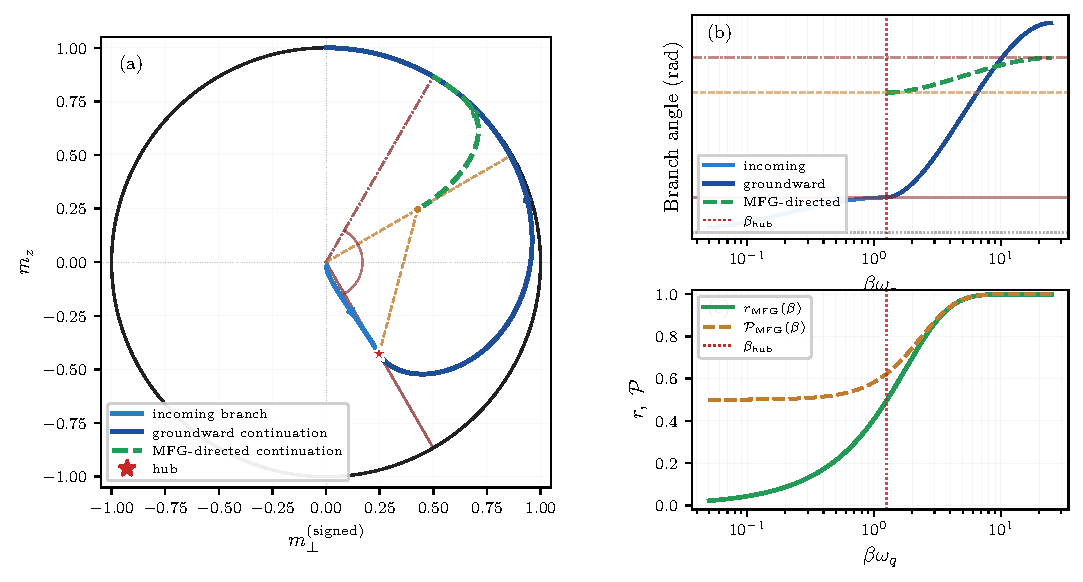
\includegraphics[width=\linewidth]{../figures/hmf_tilt_sign_mfg_branch_family}
    \caption{
    Hub-centered branch family illustrating the tilt-angle interpretation and MFG-directed continuation
    (illustrative ansatz, not an exact equilibrium trajectory).  (a) Unfolded Bloch-circle geometry in
    $(m_\perp^{(\mathrm{signed})},m_z)$: an apparent branch reaches the hub $\varphi_{\rm ax}=\pi-\theta$, after
    which one continuation returns groundward while the alternate sign/arctan image (starting at the local
    $2\theta$ point) precesses toward the coupling-direction sector $\theta$.  (b) The corresponding angle-branch
    construction.  (c) The MFG-guided Bloch radius and density-matrix purity used in the branch-family ansatz,
    $r_{\rm MFG}=\tanh[(\beta\omega_q/2)\cos\theta]$ and
    $\mathcal P_{\rm MFG}=\tfrac12(1+r_{\rm MFG}^2)$.
    }
    \label{fig:tilt_sign_mfg_branch_family}
\end{figure*}
